\begin{mainquestion}{twostage}{Two-Stage Amplifier Power Analysis}

Consider the two-stage amplifier shown below. The coupling capacitors are "shorts" at the AC frequencies of interest. $V_t = \qty{0.5}{\volt}$ and $\lambda = \qty{0.01}{\volt}^{-1}$ for both transistors.

\begin{center}
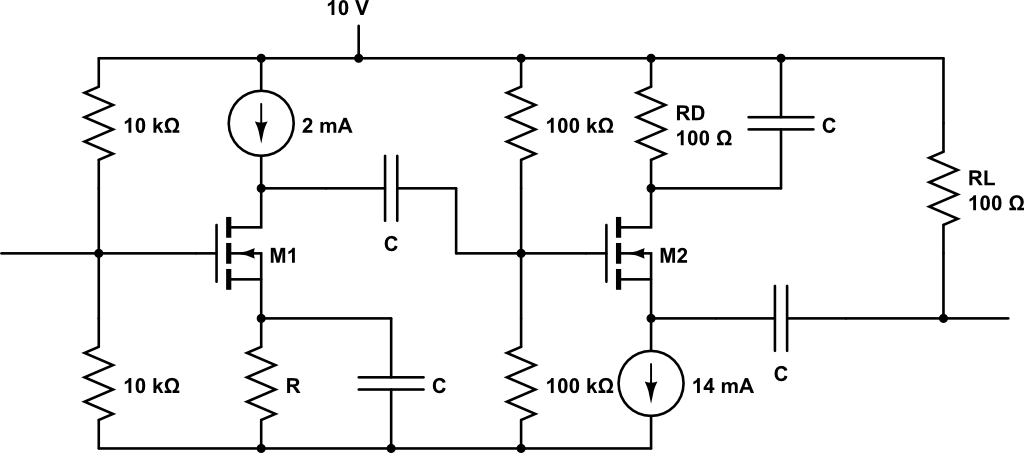
\includegraphics[width=4.5in]{image87.png}
\end{center}

\begin{partquestion}{stage1}{What is Stage 1? Assume M1 is in saturation and evaluate the voltage gain $A_{v1}$, input resistance $R_{i1}$, and output resistance $R_{o1}$ given $k_{n1} = 1\ \frac{\text{mA}}{\text{V}^{2}}$.}
\begin{answer}

The first stage is delineated in the above drawing; it is a common source amplifier.  Note the input is at the gate and the output is taken from the drain.  It is clear that the current in M1 is $I_{D1}=\qty{2}{\milli\ampere}$.  It follows that:

\[
g_{m1} = \sqrt{2 k_{n1} I_{D1}} = \sqrt{2(1)(2)} = \qty{2}{\milli\siemens}
\]

and

\[
r_{o1} = \frac{1}{\lambda I_{D1}} = \frac{1}{(0.01)(2)} = \qty{50}{\kilo\ohm}
\]

The problem reminds us that the capacitors will become shorts in our frequency of interest. Therefore, the source resistor R is not part of the small signal analysis—it is only there to provide DC biasing.  Furthermore, the DC current source becomes an open circuit in small-signal analysis. These points help codify the small-signal equivalent circuit, which is shown below.

\begin{center}
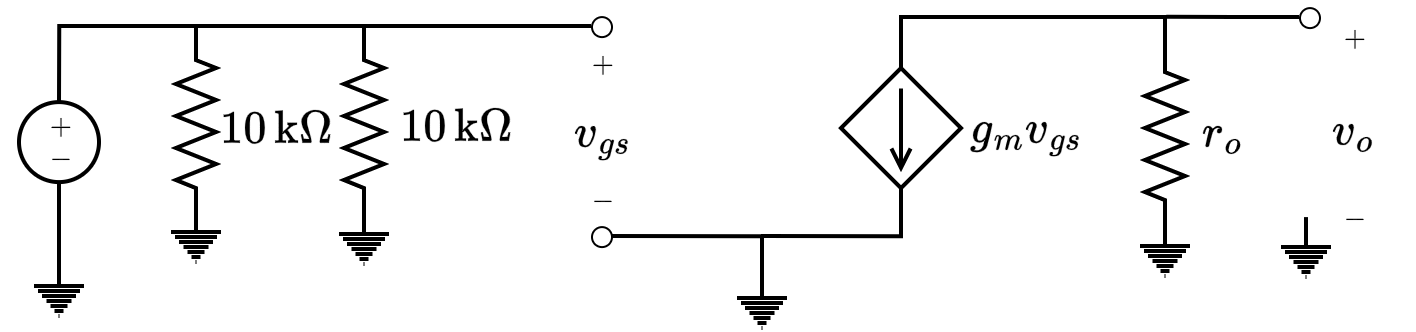
\includegraphics[width=4.5in]{pic1.png}
\end{center}

The gain of this stage is given by:
\[ A_{v1} = -g_{m1}r_{o1} = -(2)(50) = -100\]
From the circuit above, we can find the input and output resistances:
\[R_{i1} = \qty{10}{\kilo\ohm} \parallel \qty{10}{\kilo\ohm} = \qty{5}{\kilo\ohm}\]
and
\[ R_{o1} = r_{o1} = \qty{50}{\kilo\ohm}\]
\end{answer}
\end{partquestion}

\begin{partquestion}{stage2}{What is Stage 2? Assume M2 is in saturation and evaluate the voltage gain $A_{v2}$, input resistance $R_{i2}$, and output resistance $R_{o2}$ given $k_{n2} = 3\ \frac{\text{mA}}{\text{V}^{2}}$.}
\begin{answer}
The second stage is delineated in the above drawing; it is a common drain amplifier.  Note the input is at the gate and the output is taken from the source.  It is clear that the current in M2 is $I_{D2}=\qty{14}{\milli\ampere}$.  It follows that:
\[
g_{m2} = \sqrt{2 k_{n2} I_{D2}} = \sqrt{2(3)(14)} =\qty{9.165}{\milli\siemens}
\]

and

\[
r_{o2} = \frac{1}{\lambda I_{D2}} = \frac{1}{(0.01)(14)} = \qty{7.14}{\kilo\ohm}.
\]

For the AC analysis, the capacitor will be a short circuit in our frequency of interest, and the DC current source is an open circuit.  Our equivalent model is shown below:

\begin{center}
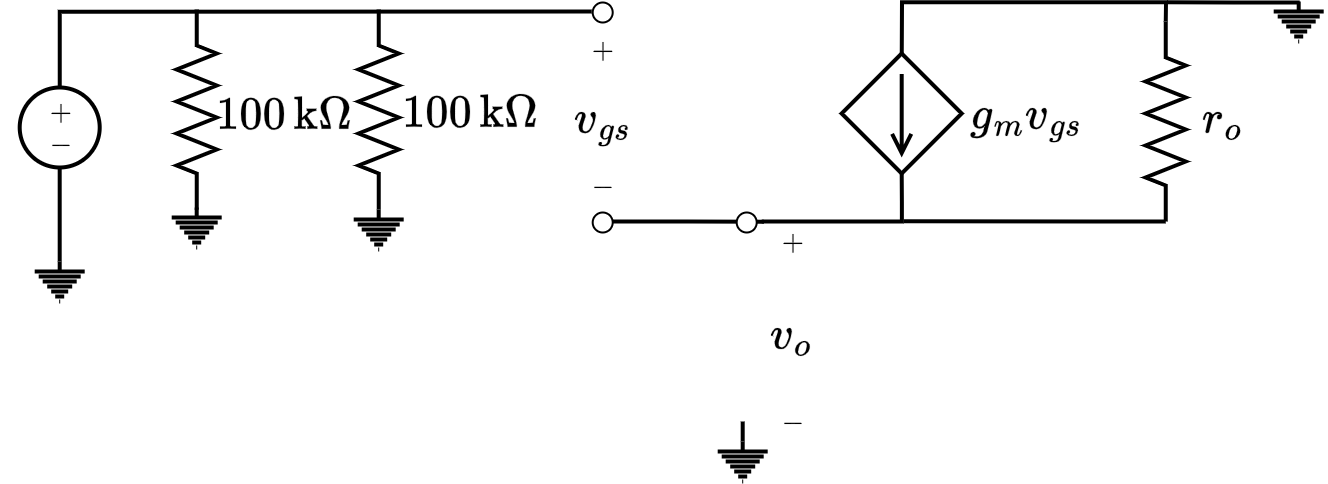
\includegraphics[width=4.5in]{pic2.png}
\end{center}

To find the gain of this stage we have:
\begin{align*}
    v_{gs} &= v_i - v_o \\
    v_o &= g_{m2}v_{gs}r_{o2} = g_{m2}(v_i - v_o)r_{o2} \\
    v_o(1 + g_{m2}r_{o2}) &= g_{m2}r_{o2}v_i\\
\end{align*}

so, it follows that:

\[
A_{v2} = \frac{v_o}{v_i} = \frac{g_{m2}r_{o2}}{1 + g_{m2}r_{o2}} = \frac{(9.165)(7.14)}{1 + (9.165)(7.14)} = 0.985
\]

The input resistance is given by the two 100 kΩ resistors:
\[R_{i2}=\qty{100}{\kilo\ohm} \parallel \qty{100}{\kilo\ohm} =\qty{50}{\kilo\ohm} \]

To find the output resistance, we short the input of the circuit and put a test source at the output, as shown below:

\begin{center}
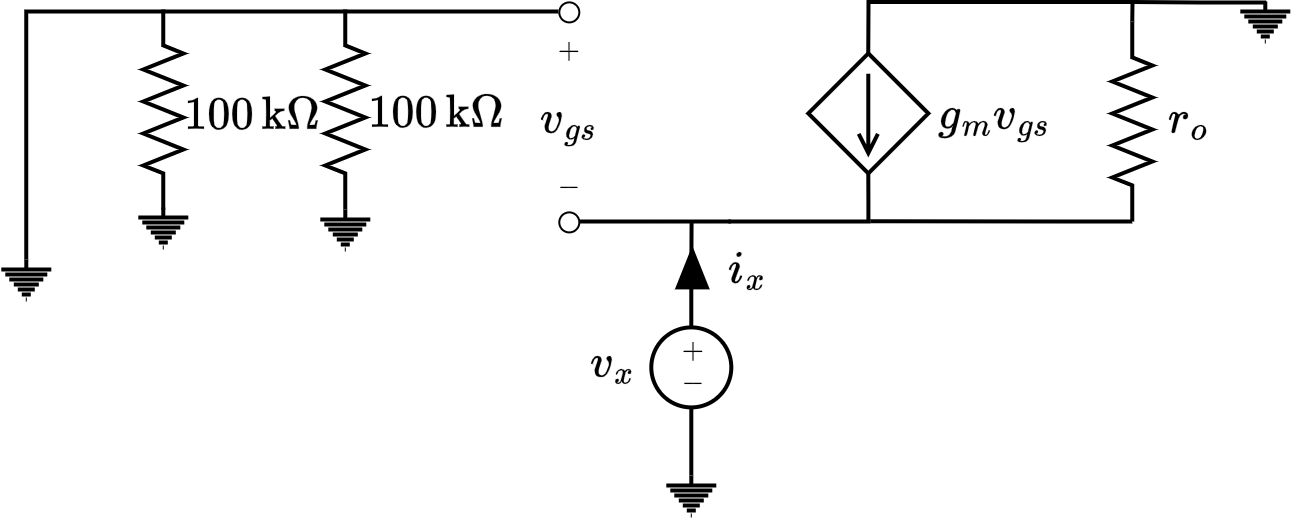
\includegraphics[width=4.5in]{pic3.png}
\end{center}

We can calculate:

\begin{align*}
v_{gs}&=0-v_{x} \\
i_{x}+g_{m2}v_{gs}-\frac{v_{x}}{r_{o2}}&=0 \\
i_{x}-g_{m2}v_{x}-\frac{v_{x}}{r_{o2}}&=0
\end{align*}
so
\[
R_{o2}=\frac{v_{x}}{i_{x}}=\frac{r_{o2}}{1+g_{m}r_{o2}}=\frac{7.14}{1+\left(9.165\right)\left(7.14\right)}=\qty{107.47}{\ohm} . 
\]
\end{answer}
\end{partquestion}

\begin{partquestion}{overallgain}{Find the overall voltage gain $\frac{v_{o}}{v_{i}}$.}
\begin{answer}

Drawing the equivalent circuit based on the results of the previous items:

\begin{center}
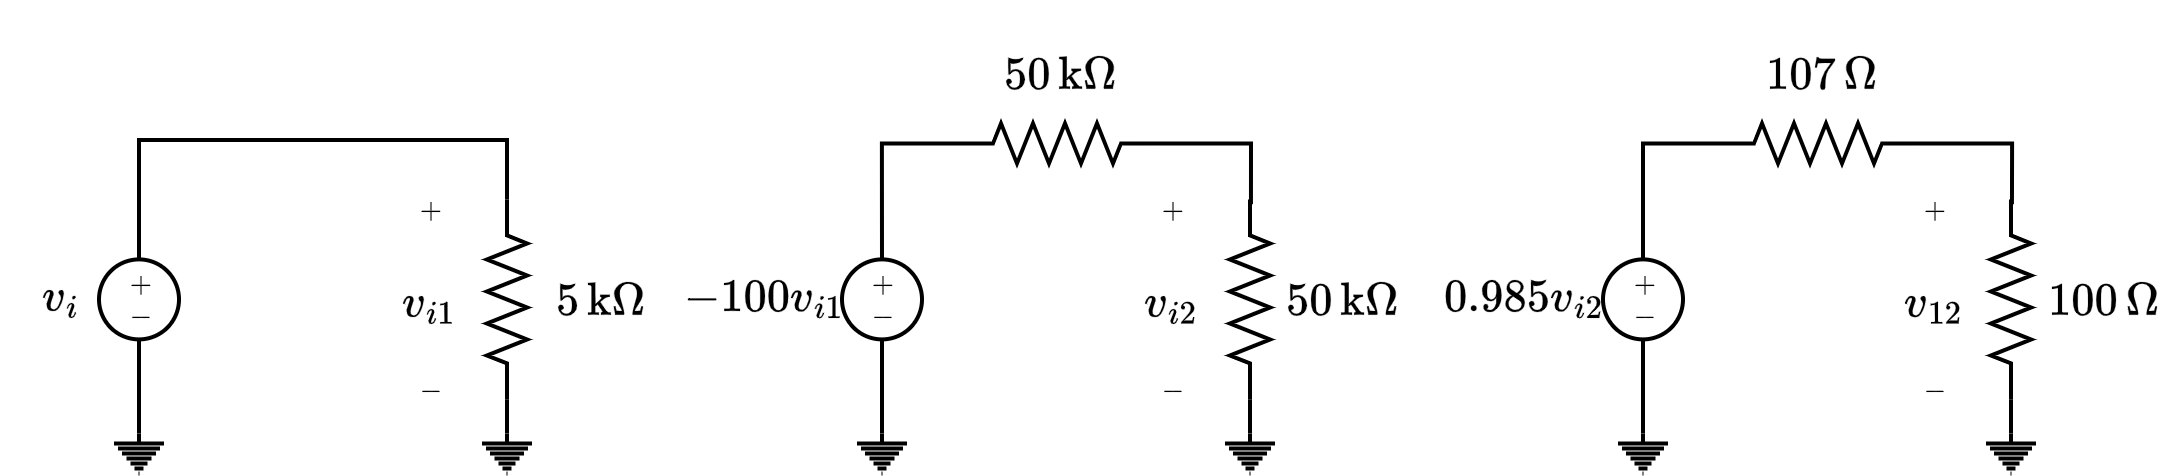
\includegraphics[width=6in]{pic5.png}
\end{center}

We can calculate:
\begin{gather*}
    v_{i1}=v_{i} \\
    v_{i2}=-100v_{i1}\frac{\qty{50}{\kilo\ohm} }{\qty{50}{\kilo\ohm} +\qty{50}{\kilo\ohm} }=-50v_{i1} \\
    v_{o}=0.985v_{i2}\frac{\qty{100}{\ohm} }{\qty{107.47}{\ohm} +\qty{100}{\ohm} }=0.4748v_{i_{2}}
\end{gather*}

So

\[
A_{v}=\frac{v_{o}}{v_{i}}=\left(0.4748\right)\left(-50\right)\left(1\right)=-23.74. 
\]
\end{answer}
\end{partquestion}

\begin{partquestion}{power}{Find the total DC power dissipated in the amplifier and the RMS power dissipated in the $\qty{100}{\ohm}$ load if the input is $v_{i}(t) = 0.01 \sin \omega t$ V. What is the ratio between this RMS output power and the total DC power?}
\begin{answer}
The DC power dissipated in the amplifier is the sum of the power dissipated in each branch, including gate bias branches. We can use the fact that each branch drops the full 10 V input
across it:
\[P_{DC}=\left(2\text{\ mA\ +\ 14\ mA}\right)\left(\qty{10}{\volt}\right)+\frac{{\left(\qty{10}{\volt}\right)}^{2}}{\qty{20}{\kilo\ohm} }+\frac{{\left(\qty{10}{\volt}\right)}^{2}}{\qty{200}{\kilo\ohm} }=165.5\text{\ mW.} \]
The RMS power dissipated in the load can be found using $v_{i}\left(t\right)$ and the total gain of the circuit:
\[P_{o,\text{RMS}}=\frac{{v_{o,\text{RMS}}}^{2}}{R_{L}}=\frac{{\left(A_{v}v_{i,\text{RMS}}\right)}^{2}}{R_{L}}=\frac{{\left(-23.74\frac{0.01}{\sqrt{2}}\right)}^{2}}{\qty{100}{\ohm} }=0.282\text{\ mW.}\]
The small-signal output power is about:
\[\frac{\qty{0.282}{\milli\watt}}{\qty{165.5}{\milli\watt}}\times 100\%=0.17\% \]
of the total dissipated DC power.  Yee-haw!
\end{answer}
\end{partquestion}

\end{mainquestion}
